\chapter{Especificación del sistema}

\section{Requisitos}
\subsection{Requisitos funcionales\label{reqF}}
\begin{itemize}
    \itemsep0em 
    \item El sistema procesará el movimiento del dispositivo resultando en la
    identificación de una letra.
    \item El sistema enviará la letra identificada por el sistema
    de comunicación pertinente a una interfaz de usuario.
    \item Al detectar un movimiento despreciable, el dispositivo lo descartará.
    \item Posterior a la identificación del movimiento, el sistema
    dejará un periodo suficiente de no registro de movimiento para
    que el usuario recoloque su postura.
    \item El sistema debe contar con un programa para ordenador, una interfaz
    gráfica que medie entre el dispositivo y el usuario.
\end{itemize}


\subsection{Requisitos no funcionales\label{reqNF}}
\begin{itemize}
    \itemsep0em
    \item El tiempo de procesamiento para la identificación de la letra,
    debe ser inmediato para generar sensación de escritura natural.
    \item El sistema debe funcionar con conexión por cable e inalámbrica.
    \item La interfaz de usuario debe ser simple de entender y usar.
    \item El sistema debe contar con autonomía energética.
    \item El dispositivo estará integrado en un encapsulado.
    \item El encapsulado tendrá un tamaño y forma semejante a un lápiz o bolígrafo.
    \item El microcontrolador debe tener unas dimensiones adecuadas pra encajar
    en el encapsulado.
    \item El producto debe estar sujeto a un presupuesto no superior a los 65€.
\end{itemize}

\section{Especificación formal}

\subsection{Especificación hardware\label{reqHW}}
El dispositivo a crear clasificará, de forma autónoma, los distintos
gestos que se realicen
como letras, usando como herramienta de procesamiento Deep Learning.
Por tanto la placa debe contar con:
\begin{itemize}
    \itemsep0em
    \item Dada la limitación de presupuesto, se optará por un microcontrolador.
    \item El microcontrolador debe ser compatible con el procesamiento de
    tensores para poder trabajar con modelos basados en \textit{Deep Learning}.
    \item Sensores presentes en el microcontrolador suficientes para hacer
    reconocible el movimiento con precisión. En su defecto, se integrarán.
    \item Microcontrolador con tecnología inalámbrica.
    \item Microcontrolador con dimensiones reducidas.
    \item Un encapsulado que le dé cabida al propio microcontrolador
    y a la batería, cableado, etc.
\end{itemize}

\subsection{Especificación software}
\begin{itemize}
    \itemsep0em
    \item Interfaz de usuario simple que ofrezca las funcionalidades
    descritas.
    \item Framework adecuado para el diseño, entrenamiento, validación y testeo
    de redes neuronales y su integración en el microcontrolador.
    \item Firmware para el microcontrolador que integre la red neuronal
    para la tarea de detección de letras y la recolección del movimiento.
    \item Un software suficiente para la creación del encapsulado.
    \item Documentación para que la comunidad pueda hacer uso del producto
    y aportar nuevas funcionalidades al proyecto.
\end{itemize}


\section{Planificación y presupuestación}
\subsection{Planificación}
La planificación ha sido esencial para poner en valor los tiempos que manejar
y ser consciente de las limitaciones.
Es lo primero que se debe plantear unido a una preparación o documentación
sobre lo que se va a trabajar para, solo de esta forma, poder estimar de una
forma más precisa los plazos de cada elemento ineludible en el desarrollo
del producto que se busca.
\begin{figure}[]
    \centering
    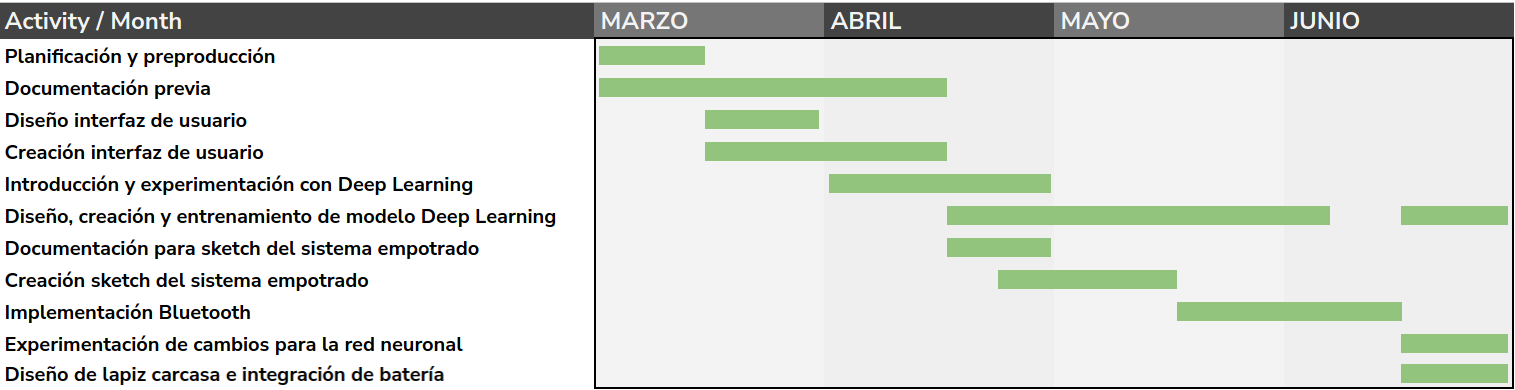
\includegraphics[angle=270,width=0.47\textwidth]{capturas/ganttFixed.png}\\[-0,20cm]
    \caption{Diagrama \textit{Gantt} para la planificación}
\end{figure}
\newpage
Como muestra la Figura 3.1, ha sido una planificación basada en contenidos, sin prácticamente iteraciones
de desarrollo, ya que, dados todos los campos que se abarcan
y dada la complejidad de alguno de ellos; es improbable poder
contar con varias iteraciones. La excepción de este precepto viene
con el modelo, con el que se tratará de experimentar, con franqueza
por apetencia de estudiar aún más las redes neuronales y su desempeño.

Por lo que podríamos clasificar el desarrollo formalmente como un modelo de prototipos;
donde se estudian los requisitos, se documenta al respecto y se crea un
prototipo revisable en caso de incumplimiento de requisitos o por
errores en la implementación que se reflejen negativamente en el prototipo.

Aunque solo encontramos esa segunda iteración o revisión en la red neuronal,
hay un cierto patrón de documentación y ejecución para cada parte del
proyecto, por lo que se podría decir que los procesos están fraccionados.
Sin embargo no deja de ser, como se ha denominado anteriormente, una
planificación basada en contenidos: se ejecuta una parte y se procede con
la siguiente.

El orden ha sido relevante y tiene su propósito. En primer lugar
está la documentación  y planificación, seguida de la creación de
la interfaz, no por otra cosa que la carencia del hardware. Estos plazos
son los primeros ya que permiten trabajar sin el sistema empotrado; tiempos
de selección y obtención del hardware. Complementariamente, el diseño
de la interfaz de usuario abre la mente a reflexionar sobre qué podría
ofrecer el dispositivo a la persona que hace uso de él, ayuda a pensar
en nuevas funcionalidades.

El siguiente bloque de contenido es el del modelo basado en
\textit{Deep Learning}, ya que si el modelo no alcanzara en la fase de
testeo unos resultados óptimos, todavía podemos contar con algo más de
tiempo para solventar su eficiencia.

Y por último la creación del propio firmware del microcontrolador y la
integración del bluetooth, dividida en la implementación en la interfaz
de usuario y en el firmware; para
poder congregar finalmente todos los elementos y probar el resultado del producto.

Una última fase de experimentación en la que también se incluirá la creación
y producción del embellecimiento para el dispositivo en forma de lápiz y la
integración de su batería en el mismo.
\newpage
\subsection{Presupuesto\label{presupuesto}}
Para esta sección ha de tenerse en consideración la situación en el momento
del desarrollo del proyecto de escasez de silicio, huelgas de transporte, pandemia,
etc. Repercutiendo directamente en el precio de la electrónica y en los tiempos de
entrega.

Aclarado esto, el presupuesto dada la naturaleza del proyecto, su funcionalidad
y que se realiza con fines académicos y experimentales; será uno limitado y
acorde a lo que se podría esperar.

En cuanto al coste del trabajo del ingeniero que lo desarrollará, se ha consultado el salario
medio de un ingeniero informático en España en 2022\cite{salII}.
El pago por hora medio ronda los 13,59€, teniendo en cuenta mi experiencia laboral y mis
conocimientos previos acerca de \textit{machine learning}, voy a
quedarme con una cifra algo más baja de 12.50€. Por lo que, teniendo en cuenta que
este proyecto ocupa 12 créditos y cada crédito equivale a unas 26h de trabajo,
este trabajo debería realizarse en unas 312 horas, lo que equivale a 3900€.

\begin{table}[h]
    \color{mitexto}
    \begin{tabular}{ll}
    \hline
    \rowcolor[HTML]{6665CD} 
    \multicolumn{1}{|l|}{\cellcolor[HTML]{6665CD}{\color[HTML]{EFEFEF} \textbf{Descripción}}} & \multicolumn{1}{l|}{\cellcolor[HTML]{6665CD}{\color[HTML]{EFEFEF} \textbf{Precio}}} \\ \hline
    \multicolumn{1}{|l|}{Microcontrolador ~~~~~~~~~~~~~~~~~~~~~~~~~~~~~~~~~~~~~~~~~~~~~~~~~~~~}& \multicolumn{1}{r|}{~~~~~~~~~~~~~~40€}                                            \\
    \multicolumn{1}{|l|}{Batería}                                                  & \multicolumn{1}{r|}{15€}                                                         \\
    \multicolumn{1}{|l|}{Adaptación batería}                                                           & \multicolumn{1}{r|}{2€}                                                             \\
    \multicolumn{1}{|l|}{Impresión del encapsulado}                                                           & \multicolumn{1}{r|}{1€}                                                          \\
    \multicolumn{1}{|l|}{Cableado}                                                           & \multicolumn{1}{r|}{7€}                                                          \\
    \multicolumn{1}{|l|}{Tiempo de trabajo}                                                           & \multicolumn{1}{r|}{3900€}                                                             \\\hline
    \multicolumn{1}{r}{\textbf{EQUIPO:}}                                                       & \textbf{65'00€} \\                                                                    
    \multicolumn{1}{r}{\textbf{TOTAL:}}                                                       & \textbf{3965'00€}                                                                    
    \end{tabular}
    \caption{Presupuesto estimado para la producción}
\end{table}